\chapter{CONVECCIÓN FORZADA}

\begin{figure}[!h]
\centering
\includegraphics[scale=1.90]{figura05_01.eps}
\end{figure}

\begin{table}[!h]
\begin{center}
\begin{tabular}{|m{6.8cm}
                |m{6.8cm}|}
\hline
\textbf{Ventajas} &
\textbf{Desventajas} \tabularnewline \hline
Disminución del tiempo de proceso. &
Inversión en equipamiento. \tabularnewline \hline
Permite el manejo de grandes volúmenes. &
Gasto de energía para un sistema mecánico. \tabularnewline \hline
Transmisión de elevadas tasas de calor. &
Gasto de mantenimiento. \tabularnewline \hline
Uso industrial. & \tabularnewline \hline
\end{tabular}
\end{center}
\end{table}

\begin{equation*}
    q = h_{CF}\,A\,\Delta t
\end{equation*}

Donde $h_{CF}$, es el coeficiente de convección forzada, que es mayor al
coeficiente de convección natural.
\begin{equation*}
    h_{CF} > h_{CN}
\end{equation*}

\section{Calculo de $h$}
\underline{Casos}:
\begin{enumerate}
    \item Tubos únicos.
    \begin{enumerate}
        \item Flujo por el interior.
        \item Flujo por el exterior.
    \end{enumerate}
    \item Conjunto de tubos.
    \begin{enumerate}
        \item Método de \emph{Crimson} (Coeficiente externo).
    \end{enumerate}
\end{enumerate}

\underline{Tipos de régimen}:
\begin{itemize}
    \item Régimen laminar.
    \item Régimen turbulento.
\end{itemize}

\underline{Número de \emph{Reynolds}}:
\begin{equation}
    \text{Re} = \frac{v\,D\,\rho}{\mu}
\end{equation}

\section{Caso: Interior de tubos}
\begin{equation*}
    \rho = \frac{m}{V}
\end{equation*}
\begin{equation*}
    m = V\,\rho
\end{equation*}
\begin{equation*}
    \dot{m} = v\,A_T\,\rho
\end{equation*}
\begin{equation*}
    v\,\rho = \frac{\dot{m}}{A_T} = G
\end{equation*}

\begin{equation}
    \text{Re} = \frac{G\,D_I}{\mu}
\end{equation}

Donde:
\begin{itemize}
    \item $D_I$: Diámetro interno (Longitud característica).
    \item $A_T$: Sección transversal del tubo.
    \item $G$: Flujo másico por sección transversal.
\end{itemize}

Si:
\begin{itemize}
    \item $\text{Re} \le 2100$, el régimen es \textbf{laminar}.
    \item $\text{Re} > 2100$, el régimen es \textbf{turbulento}.
\end{itemize}

\subsection{Caso: Tubo único, flujo interior, régimen turbulento}
Se utiliza las ecuaciones de \emph{Dittus}-\emph{Boelter}:

\begin{equation}
    \text{Nu}_F = 0.023\,\text{Re}^{0.8}\,\text{Pr}^{0.33}
    \label{dittus1}
\end{equation}
\begin{equation}
    \text{Nu} = 0.023\,\text{Re}^{0.8}\,\text{Pr}^{0.4}
    \quad\text{(Calentamiento)}
    \label{dittus2}
\end{equation}
\begin{equation}
    \text{Nu} = 0.023\,\text{Re}^{0.8}\,\text{Pr}^{0.3}
    \quad\text{(Enfriamiento)}
    \label{dittus3}
\end{equation}

\begin{figure}[!h]
\centering
\includegraphics[scale=2.00]{figura05_02.eps}
\caption{Sección de un tubo.}
\end{figure}

Para (\ref{dittus1}), las propiedades se calculan a la temperatura de película:
\begin{equation*}
    t_\text{F} = \frac{t_\text{INT} + \bar{t}_{\infty}}{2}
\end{equation*}

Para (\ref{dittus2}) y (\ref{dittus3}), las propiedades se calculan a la
temperatura media del fluido:
\begin{equation*}
    \bar{t}_\infty = \frac{t_1 + t_2}{2}
\end{equation*}

Donde:
\begin{itemize}
    \item $t_\text{INT}$: Temperatura de la superficie interna.
    \item $\bar{t}_\infty$: Temperatura media o global del fluido.
\end{itemize}

\subsubsection{Caso: Gases}
$\text{Pr} = 0.74$ es un valor constante.
\begin{equation}
    \text{Nu} = 0.021\,\text{Re}^{0.8}
\end{equation}

\subsubsection{Caso: Flujo isotérmico (vapor)}
\begin{equation}
    h = 0.023\,
    \left(\frac{G^{0.8}}{D^{0.2}}\right)
    \left(\frac{Cp^{0.4}\,k^{0.6}}{\mu^{0.4}}\right)
\end{equation}

\subsubsection{Caso: Fluido muy viscoso ($\text{Re} \le 8000$)}
Se usa la ecuación de \emph{Sieder} y \emph{Tate}:
\begin{equation}
    \text{Nu} = 0.027\,\text{Re}^{0.8}\,\text{Pr}^{0.333}\,
    \left(\frac{\mu}{\mu_S}\right)^{0.14}
\end{equation}

Donde:
\begin{itemize}
    \item $\mu$: Viscosidad a la temperatura media del fluido.
    \item $\mu_S$: Viscosidad a la temperatura de superficie.
\end{itemize}

\subsection{Caso: Tubo único, flujo interior, régimen laminar}
La ecuación general es:

\begin{equation}
    \text{Nu} = 2.0\,
    \left(\frac{W\,Cp}{k\,L}\right)^{\frac{1}{3}}
    \left(\frac{\mu}{\mu_S}\right)^{0.14}
\end{equation}

Donde:
\begin{itemize}
    \item $W$: Flujo másico $[kg/h]$.
    \item $L$: Longitud del tubo $[m]$.
\end{itemize}

\subsubsection{Caso: Agua}
En este caso $\mu$ es constante, por tanto:

\begin{equation*}
    \frac{\mu}{\mu_S} = 1.0
\end{equation*}

\section{Caso: Flujo por el exterior de tubos}

\subsection{Caso: Régimen turbulento}
Para líquidos:
\begin{equation}
    \text{Nu}_\text{F} = \text{Pr}_\text{F}^{0.3}\,
    (0.35+0.47\text{Re}_\text{F}^{0.52})
\end{equation}

Para gases:
\begin{equation}
    \text{Nu}_\text{F} = 0.26\,\text{Pr}_\text{F}^{0.3}\,
    \text{Re}_\text{F}^{0.6}
\end{equation}

Las propiedades se calculan a la temperatura de película:
\begin{equation*}
    t_\text{F} = \frac{t_\text{WE} + \bar{t}_{\infty}}{2}
\end{equation*}
\begin{equation*}
    \bar{t}_\infty = \frac{t_i + t_o}{2}
\end{equation*}

\subsubsection{Caso: Aire y gases diatómicos}
\begin{equation}
    \text{Nu} = 0.32 + 0.43\,\text{Re}^{0.52}
\end{equation}
\begin{equation*}
    \text{Nu} = 0.45 + 0.33\,\text{Re}^{0.56}
\end{equation*}
\begin{equation*}
    \text{Nu} = 0.24\,\text{Re}^{0.6}
\end{equation*}

\subsubsection{Caso: Cambiadores de calor de doble tubo o tubos concéntricos}
\begin{figure}[!h]
\centering
\includegraphics[scale=2.00]{figura05_03.eps}
\caption{Sección de dos tubos concéntricos.}
\end{figure}

Se utiliza la ecuación de \emph{Davis}:
\begin{equation}
    \frac{h}{Cp\,G} = 0.029\,
    \left(\frac{D_\text{I}\,G}{\mu}\right)^{-0.2}
    \left(\frac{C_p\,\mu}{k}\right)^{-\frac{2}{3}}
    \left(\frac{\mu}{\mu_s}\right)^{0.14}
    \left(\frac{D_\text{E}}{D_\text{I}}\right)^{0.25}
\end{equation}
\begin{equation*}
    \frac{h}{Cp\,G} = 0.029\,
    \text{Re}^{-0.2}\,
    \text{Pr}^{-\frac{2}{3}}
    \left(\frac{\mu}{\mu_s}\right)^{0.14}
    \left(\frac{D_\text{E}}{D_\text{I}}\right)^{0.25}
\end{equation*}

Donde:
\begin{itemize}
    \item $D_\text{I}$: Diámetro interno de la zona anular.
    \item $D_\text{E}$: Diámetro externo de la zona anular.
\end{itemize}

Si, alguno de los tubos tiene un diámetro variable, se debe usar el valor del
perímetro, de la siguiente manera:
\begin{equation*}
    P = \pi\,D_\text{I}
\end{equation*}
\begin{equation*}
    D_\text{I} = \frac{P}{\pi}
\end{equation*}

Por ejemplo para un tubo cuadrado seria:
\begin{equation*}
    D_\text{I} = \frac{4\,l}{\pi}
\end{equation*}

\subsection{Caso: Régimen laminar}

\subsubsection{Caso: Líquidos ($0.1 < \text{Re} < 200$)}
\begin{equation}
    \text{Nu}_\text{F} = 0.86\,\text{Pr}_\text{F}^{0.3}\,
    \text{Re}_\text{F}^{0.43}
\end{equation}

\subsubsection{Caso: Líquidos ($\text{Re} > 200$) y
Gases ($0.1 < \text{Re} < 1000$)}
\begin{equation}
    \text{Nu}_\text{F} = \text{Pr}_\text{F}^{0.3}\,
    (0.35 + 0.47\,\text{Re}_\text{F}^{0.52})
\end{equation}

\subsubsection{Caso: Aire}
\begin{equation}
    \text{Nu}_\text{F} = 0.24\,\text{Re}^{0.6}
\end{equation}

\section{Caso: Flujo por el exterior de haces de tubos}
Se consideran dos tipos de arreglos:

\begin{enumerate}
    \item En linea o cuadrangular.
    \item Escalonado, triangular o al tres bolillo.
\end{enumerate}

\begin{figure}[!h]
\centering
    \begin{minipage}{.4\textwidth}
        \centering
        \includegraphics[scale=1.00]{figura05_04.eps}
        \caption{Arreglo en linea}
    \end{minipage}
    \begin{minipage}{.4\textwidth}
        \centering
        \includegraphics[scale=1.00]{figura05_05.eps}
        \caption{Arreglo escalonado}
    \end{minipage}
\end{figure}

\subsection{Método de \emph{Crimson}}
\begin{equation}
    \text{Nu} = C\,\text{Re}_\text{max}^n
\end{equation}

Donde:
\begin{itemize}
    \item $C$, $n$, se extraen de la tabla $7-7$ del libro ``Transferencia de
        Calor'', de \emph{Pitts}.
\end{itemize}

\begin{equation}
    \text{Re}_\text{max} = \frac{v_\text{max}\,D_E}{\nu}
\end{equation}

Donde:
\begin{itemize}
    \item $v_\text{max}$: Velocidad máxima en el pasaje mínimo $[m/s]$.
    \item $D_E$: Diámetro externo $[m]$.
    \item $\nu$: Viscosidad cinemática $[m^2/s]$.
\end{itemize}

Para un arreglo en linea, se tiene:
\begin{figure}[!h]
\centering
\includegraphics[scale=2.00]{figura05_06.eps}
\end{figure}

\begin{equation}
    P_\text{min} = a - D
\end{equation}
\begin{equation}
    v_\text{max} = \frac{V_\infty\,a}{a - D}
\end{equation}

Para un arreglo escalonado, se tiene:
\begin{figure}[!h]
\centering
\includegraphics[scale=2.00]{figura05_07.eps}
\end{figure}

\begin{equation}
    P_\text{min1} = \frac{a - D}{2}
\end{equation}
\begin{equation}
    P_\text{min2} = \sqrt{\left(\frac{a}{2}\right)^2 + b^2} - D
\end{equation}
\begin{equation}
    v_\text{max} = \frac{V_\infty\,(a/2)}{\text{min}(P_\text{min1}, P_\text{min2})}
\end{equation}

Para 10 o mas tubos se obtiene el coeficiente de convección en dirección de la
corriente:
\begin{equation*}
    h_o = \frac{\text{Nu}\,k}{D}
\end{equation*}

Para menos de 10 tubos en la dirección de la corriente, se debe corregir con el
factor que se encuentra en la tabla $7-8$ del libro ``Transferencia de
Calor'', de \emph{Pitts}.

